\chapter{逆动力学} \label{chap:chap8}

任何作用力都会产生一个大小相等的反作用力。

\begin{flushright}
	——艾萨克$\cdot$牛顿爵士
\end{flushright}

\begin{figure}[!htb]
	\centering
	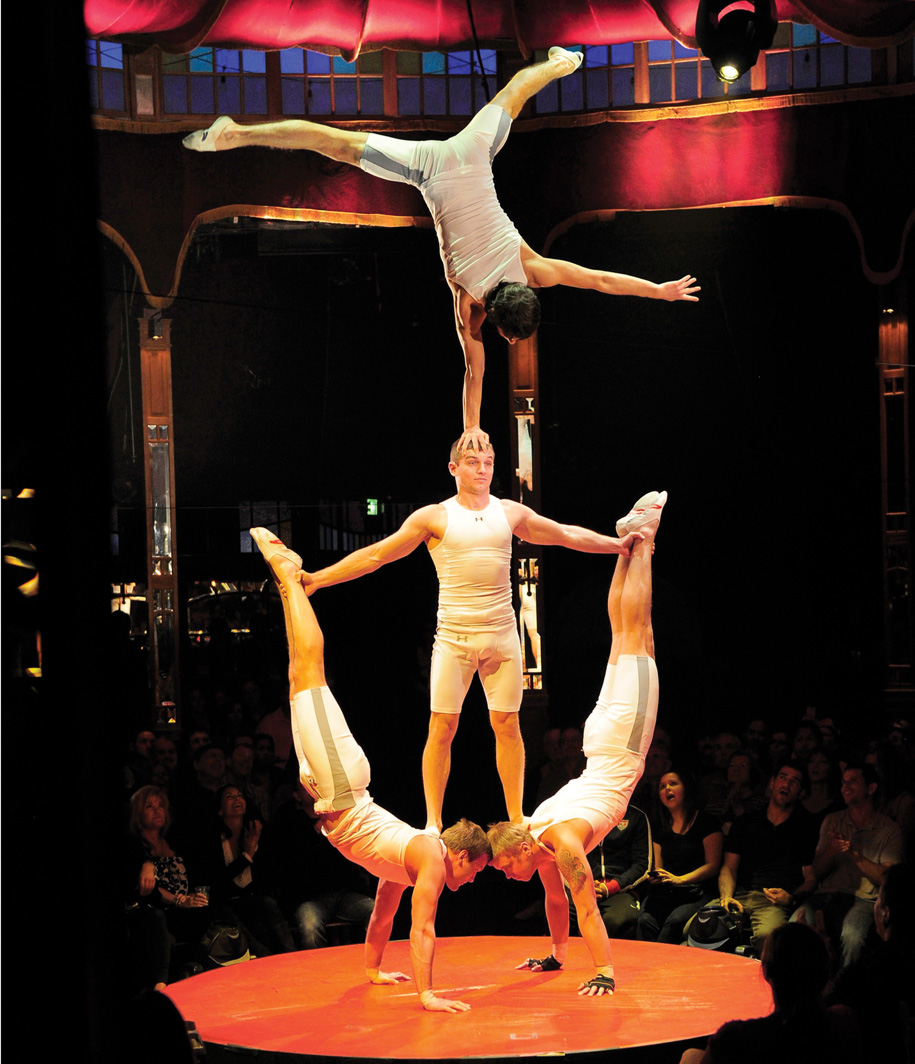
\includegraphics[width=1.0\linewidth]{chap8/8_0}
	% 加星号(*)表示不加编号
	\caption*{ \label{fig:8_0}}
\end{figure}


我母亲75岁时,几乎已经无法行走。
她的右膝每走一步都疼痛难忍,爬楼梯更是不可能。疼痛难忍。
她想和我的孩子们一起玩,却跟不上他们。
无法行走不仅限制了她的生活参与,还给她带来了心理上的创伤。
膝盖X光检查显示,她患有严重的骨关​​节炎,这是一种影响美国超过3000万人的退行性关节疾病(图~\ref{fig:8_1})。


\begin{figure}[!htb]
	\centering
	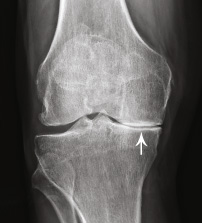
\includegraphics[width=0.4\linewidth]{chap8/8_1}
	\caption{膝盖X光片显示骨关节炎的迹象。
		请注意,膝盖内侧的骨头相互接触(见箭头);
		外侧保留了更多的软骨,表现为股骨和胫骨之间的间隙。
		图片由Julie Thompson-Kolesar提供。 \label{fig:8_1}}
\end{figure}


骨关节炎是由于覆盖骨骼末端的软骨表面磨损而引起的。
软骨很滑,没有痛觉,因此它是一种极好的材料,可以让我们的关节自由活动,而我们却感觉不到任何疼痛。
然而,当软骨磨损时,会暴露出下面的骨骼,而骨骼对压力极其敏感,会产生更大的摩擦力,导致关节感到疼痛和僵硬。


膝盖负荷过重会导致磨损,最终引发骨关节炎,然而,如果不进行手术安装传感器,就无法测量关节内的负荷。
目前只有少数勇敢的患者因其他原因接受了手术,才得以实现这一目标。
因此,我们通常采用其他方法来估算关节内的负荷。
求解逆动力学问题可以提供一些估算关节接触负荷所需的信息,这是理解生物关节失效原因的关键一步。


当工程产品发生故障时,法医工程师会努力查明故障的根本原因,并最终追究相关人员的法律责任。
例如,律师事务所会聘请精通生物力学的法医工程师,评估车辆碰撞后伤害索赔的合法性。
轮胎滑痕等物证可以用来估算碰撞过程中的力和加速度。
事故重建过程就是逆问题的一个例子,因为人们会使用间接观测来研究无法直接测量的现象。


在第~\ref{chap:chap7}~章中,我们介绍了逆运动学问题,其中一个例子是通过测量安装在皮肤上的光学标记在全局参考系中的位置来确定受试者骨骼的姿态。
在那一章中,我们的目标很有限;我们只是在回答这个问题:发生了什么?
换句话说,为了产生观察到的标记轨迹,必须存在哪些关节角度?
在本章中,我们将深入探究:是什么导致了这一切?
具体来说,是什么力和力矩导致了观察到的运动?


从运动学中确定力和力矩的过程称为逆动力学。
它与逆运动学不同,因为我们感兴趣的是产生运动的力,而不仅仅是运动本身。
它也不同于正向动力学,在正向动力学中,我们预测当指定的力施加到系统上时将产生的运动。


逆动力学问题可以通过几种方法求解。
通常,如果可以测量地面反作用力,我们会使用测量数据,因此我们将首先简要讨论测量这些力的技术。
然后,我们将展示一个详细的例子,说明如何计算深蹲过程中的关节力矩。
在这个例子中,我们从地面向上进行计算,使用地面反作用力的测量数据,并将这些信息通过腿部关节向上传递。
如果我们拥有所有身体部位运动的可靠测量数据,也可以从上向下进行计算。


请注意,本章计算的力并非生物关节中实际测量的力。
为了计算关节接触载荷,我们还必须估算肌肉施加的力。
这是一个非同小可的问题,将是第九章的重点。
目前,只需注意,相同的运动和外力可能会因肌肉协调策略的差异而产生不同的测量结果,从而产生不同的关节接触载荷(但逆动力学问题的解是相同的)。


有趣的是,如果我们能够获取地面反作用力以及所有身体部位的运动,就能得到一个超定方程组。
在这种情况下,我们可以利用这些额外的信息来最小化测量误差的影响,这一策略与第~\ref{chap:chap7}~章中描述的约束逆运动学算法相呼应。
本章最后将以一个例子来结束,该例子展示了如何利用逆动力学分析来评估膝关节骨关节炎患者的非手术治疗。
如果我早二十年想到这个方法,或许就能帮助到我的母亲。



\section{测量外力}

牛顿的三大运动定律,最早发表于他1687年出版的里程碑式著作《自然哲学的数学原理》(Philosophiæ naturalis principia mathematica)中。
牛顿第二定律是迄今为止最重要的方程之一;
安德鲁$\cdot$莫特于1729年从拉丁文原文翻译了该定律,其表述如下:


定律二:运动的改变总是与所施加的动力成正比;并且是沿着施加该力的直线方向进行的。


换句话说,粒子动量的变化率等于作用力的矢量和,方向与作用力的方向一致。
牛顿第二定律现在通常被称为 $\underline{F} = m \underline{a}$,其中$\underline{F}$是作用于物体的所有力的矢量和,$m$是物体的质量,$\underline{a}$是其质心的(线性)加速度。
这个版本遵循原始版本,前提是物体的质量在运动过程中保持不变,这在大多数应用中都是合理的。
(火箭技术是一个显著的例外。)
莱昂哈德$\cdot$欧拉后来将牛顿定律扩展到旋转运动。
欧拉第二定律告诉我们,物体绕其质心的角动量的变化率等于作用于该点的所有矩之和。
(有关正式的数学表述,请参见下面的公式~ 8.6。)


如果已知每个身体部位的质量和加速度,我们可以使用牛顿定律和欧拉定律来确定施加在每个身体上的力和力矩。
根据所研究的运动,可能会有外力作用于主体,例如重力、空气阻力或地面反作用力。
这些外力出现在主体的自由体图中,必须进行测量或估算。
在大多数人体运动情况下,忽略空气阻力并使用重力加速度 $g = 9.81 m/s^2$ 来计算重量是合理的。
我们通常倾向于尽可能测量地面反作用力和其他接触力,以提高计算的准确性,如下所示。


19 世纪末,Étienne-Jules Marey 和他的学生 Gaston Carlet 设计了第一批用于测量足部与地面接触力的装置。
通过将压力传感器嵌入鞋底,Marey 和 Carlet 能够估算出步态过程中足部与地面之间施加的力。
Carlet 的博士论文首次报告了步行过程中地面反作用力特有的双峰垂直分量,该论文发表于 1872 年——同年,利兰$\cdot$斯坦福聘请 Eadweard Muybridge 确定马匹在小跑时是否完全腾空(见图~\ref{fig:7_1})。
我发现,现代生物力学最重要的两个定量工具竟然是由两位几乎完全不知道对方在做什么的研究人员(Carlet 和 Muybridge)同时开发的,这真是令人惊叹。


在现代实验中,地面反作用力是使用一个或多个测力板来测量的:由负载传感器支撑的平坦刚性平台(图~\ref{fig:8_2})。
负载传感器包含应变计或压电晶体,可将平台的微小位移转换为电压。
虽然测力板有点像普通的弹簧式体重秤,但它们在精度、速度和数据丰富度方面存在很大差异。
由于地面反作用力变化迅速,尤其是在脚着地时,因此数据通常以每秒数千次测量的速率收集。
测力板的每个角附近通常都有一个负载传感器,每个负载传感器测量应变并报告沿三个正交轴的力。
因此,测力板有 12 个独立的力测量值,而不是像体重秤那样只有一个,这些测量值可以组合起来计算相对于测力板原点的合力和力矩。


\begin{figure}[!htb]
	\centering
	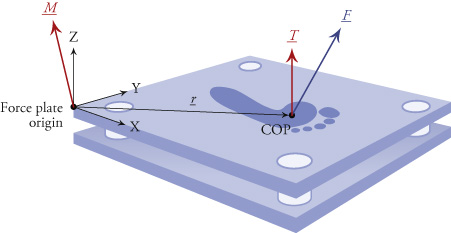
\includegraphics[width=0.7\linewidth]{chap8/8_2}
	\caption{测力台测量施加于地面和受试者之间的力和力矩,统称为地面反作用力。压力中心 (COP) 和“自由力矩” ($\underline{T}$) 可以通过合力 ($\underline{F}$) 和总力矩 ($\underline{M}$) 计算得出。 \label{fig:8_2}}
\end{figure}



\section{压力中心}

足底的压力分布不均匀(图~\ref{fig:8_3})。
这种分布的压力可以表示为施加于压力中心点的等效合力。
我们可以使用以下矩等效方程来确定压力中心:

\begin{figure}[!htb]
	\centering
	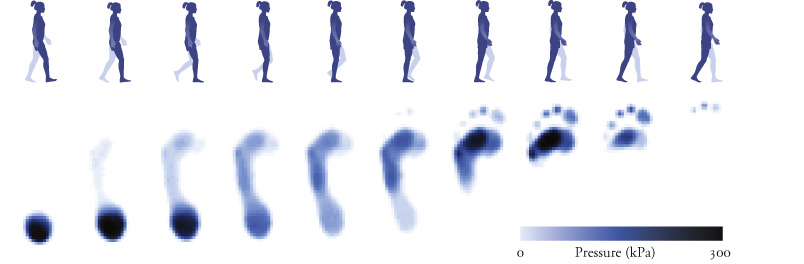
\includegraphics[width=1.0\linewidth]{chap8/8_3}
	\caption{行走时足部压力分布\cite{pataky2012gait}。 \label{fig:8_3}}
\end{figure}

\begin{equation}
	\underline{M} = \underline{r} \times \underline{F} + \underline{T}
	\label{eq:8_1}
\end{equation}
%
其中,$\underline{M}$表示测力板原点处的力矩,$\underline{r}$表示从原点到压力中心的矢量,$\underline{F}$表示合成的地面反作用力,$\underline{T}$表示在压力中心施加力时产生等效系统所需的力矩(图~\ref{fig:8_2})。
在公式~\ref{eq:8_1}~中,我们有 3 个独立方程(分别表示 $M_x$、$M_y$ 和 $M_z$),但有 6 个未知数:
矢量的 3 个分量和力矩的 3 个分量。
我们注意到压力中心保持在测力板表面($r_z = 0$),并且表面摩擦只能产生绕垂直轴的力矩($T_z$,也称为“自由力矩”),从而得到了三个附加方程。
虽然可以想象绕其他两个轴的力矩,但只有将人的脚粘在测力板上才能观察到这些力矩。
这样,脚粘的受试者才有可能产生向下的地面反作用力,从而绕其他两个轴产生力偶。


在没有粘脚的情况下,我们可以将$r_z = T_x = T_y = 0$代入公式~\ref{eq:8_1},并求解其余未知数。
我们得到压力中心相对于力板原点的位置($\underline{r}$)和自由矩($T_z$)的以下表达式:
%
\begin{equation}
	\underline{r} = 
		\begin{bmatrix}
			- M_y / F_z \\
			M_x / F_z \\
			0
		\end{bmatrix}
	\label{eq:8_2}
\end{equation}

\begin{equation}
	T_z = M_z - r_x F_y + r_y F_x
	\label{eq:8_3}
\end{equation}


在验证数据处理算法时,计算并可视化压力中心非常有用;
如果压力中心位于足迹之外,则表明测力板和运动捕捉系统之间存在校准误差。
通常,将作用于足部的力和力矩转换为压力中心,也更容易理解。
请注意,当地面反作用力 ($F_z$) 的法向分量趋近于零时,公式~\ref{eq:8_2}~中的表达式会变得病态,因此在足部触地和足尖离地附近计算出的压力中心将不可靠。



\section{逆动力学算法}

动力学分析考虑物体的运动(运动学)以及导致该运动并由该运动产生的力(动力学)。
在本节中,我们将考虑一个典型的逆动力学问题:给定一个受试者的代表性模型、受试者随时间变化的关节运动学以及施加于受试者的外力测量值,求出产生给定运动所必需的净关节力和力矩。
简而言之,我们将力学定律应用于模型中的每个身体部位,并计算作用于每个关节的内部力和力矩。
关节角度通常使用逆运动学算法(第~\ref{chap:chap7}~章)根据光学标记轨迹估算,然后对其进行平滑和微分以获得角速度和角加速度。
无需测量外力即可进行逆动力学分析,但我们将把这方面的讨论推迟到本章的后面。
为了演示一个简单的逆动力学算法,我们将计算图~\ref{fig:8_4}~所示的深蹲过程中的净关节力和力矩。


\begin{figure}[!htb]
	\centering
	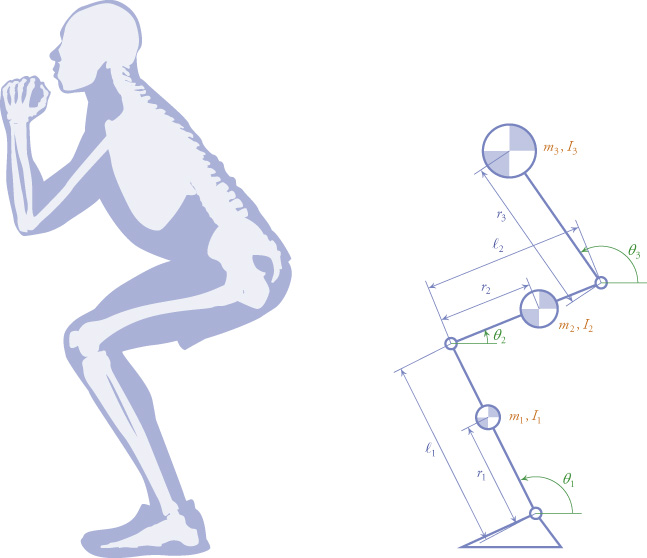
\includegraphics[width=1.0\linewidth]{chap8/8_4}
	\caption{用于研究深蹲的实验装置(左)和近似矢状面模型(右)。
		逆动力学分析根据每个身体部位的质量、惯性、几何形状和运动学参数(位置、速度和加速度)(以及外力,如有)计算每个关节处的净力和力矩。 \label{fig:8_4}}
\end{figure}


在继续之前,值得考虑一个重要问题:如何为特定研究选择合适的模型,具体来说,图~\ref{fig:8_4}~所示的简单模型是否适合研究深蹲。
一般来说,适当的模型保真度(即模型代表现实的程度)取决于所研究的问题。
重要的是要认识到,更详细的模型并不一定更好。
选择模型的目标是最大化模型的效用,这通常涉及最小化其复杂性,以使模拟结果不被无关细节所污染。
这一目标呼应了爱因斯坦 1934 年的论文《论理论物理方法》中的以下智慧:


不可否认的是,所有理论的最高目标都是使不可简化的基本要素尽可能简单、尽可能少,同时又不必放弃对单一经验数据的充分表示。


爱因斯坦谈论的是理论物理学和实验物理学之间的关系,但这里也秉持着同样的理念:
我们倾向于那些复杂程度最低、同时能够解释实验观测结果并以足够高的精度产生所需输出的模型。
正如统计学家乔治$\cdot$博克斯和诺曼$\cdot$德雷珀的名言所说:“所有模型都是错误的,但有些模型是有用的。”


一个特定模型是否有用,而不是仅仅有误,取决于它的使用环境。
例如,在模拟太阳系中的行星轨道或预测行星际航天器的轨迹时,将火星建模为点质量可能是合理的,但这样的模型不足以研究火星的天气模式或模拟航天器在那里着陆。
相反,在轨道力学研究中使用详细的行星模型会增加建模的复杂性和计算工作量,而不会增加结果的价值。
回到生物力学领域,我们注意到,一些 OpenSim 软件的新用户最初认为他们应该始终使用具有数十个自由度的全身模型,而实际上一个简单得多的模型就可以告诉他们关于他们感兴趣的特定主题所需的一切信息。
只能屈曲和伸展的单自由度膝关节模型可能适合研究膝关节伸展力矩如何随跑步速度而变化,而分析骨关节炎患者的额平面力矩则需要具有更多自由度的更详细的膝关节模型。



\section{具有地面反作用力的逆动力学}


在本节中,我们将使用图~\ref{fig:8_4}~所示的平面模型,对双腿下蹲的某一瞬间进行逆动力学分析。
该模型由四个刚体组成,它们通过三个旋转(销)关节连接,分别代表踝关节、膝关节和髋关节。
我们假设关节角度、角速度和角加速度已通过先前求解逆运动学问题获得。
我们进一步假设受试者的身体是对称的,并且任何超出矢状面的运动都可以忽略不计。
我们将左右脚组合成一个刚体(“脚”),假设其质量可忽略不计,并在地面上保持静止。
左右小腿也组合成一个刚体,其质量和惯性分别代表两个小腿;左右大腿也以类似的方式组合。
我们将头部、手臂和躯干(HAT)建模为一个刚体。
我们假设模型的每个身体部位都经过适当缩放,以匹配受试者相应身体部位的尺寸和质量特性。
在实践中,模型参数(例如长度、质量和惯性)可以通过结合直接测量、已发表的人体测量表、照片、医学图像以及其他测量和估算技术来确定。
我的团队开发的 OpenSim 模型包含这些参数的值,这些值可以缩放以代表特定个体。
我们的模型可免费获取,可从本书网站访问。


在这个简单的例子中,我们将从脚部开始,利用运动定律,借助一系列自由体运动图,计算从脚踝开始的每个关节所受的净力和力矩。
目前,我们假设地面反作用力已知。
对于像这样的简单模型,绘制自由体运动图并进行手算的策略已经足够;
在实践中,我们通常使用与下文类似的算法的软件实现。


我们假设尺寸和地面反作用力已知,并且双足无质量且静止不动。
因此,在足部自由体受力分析图(图~\ref{fig:8_5})中唯一未知的就是施加于踝关节的力和力矩。
注意,根据牛顿第三运动定律,作用于小腿踝关节的力和力矩必须大小相等、方向相反。
我们习惯于在较近端的小腿上绘制这些矢量对的正方向,在较远端的小腿上绘制这些矢量对的负方向。
例如,图~\ref{fig:8_5}~中的 $F_{x_1}$ 矢量指向 -X 方向,则小腿自由体受力分析图(图~\ref{fig:8_6})中对应的矢量将指向 +X 方向。


\begin{figure}[!htb]
	\centering
	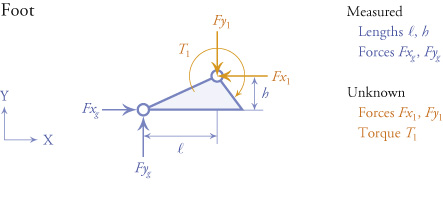
\includegraphics[width=0.7\linewidth]{chap8/8_5}
	\caption{模型足部段的自由体受力图如图~\ref{fig:8_4}~所示。 \label{fig:8_5}}
\end{figure}


\begin{figure}[!htb]
	\centering
	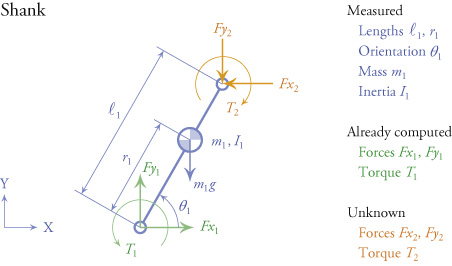
\includegraphics[width=0.7\linewidth]{chap8/8_6}
	\caption{图~\ref{fig:8_4}~所示模型小腿段的自由体图。
		自由体图中身体段的姿势无需与其在研究活动中的姿势一致。
		虽然数学上无关紧要,但我们以这个方便的标准姿势绘制小腿段,其中 1 介于 0 到 90 度之间。 \label{fig:8_6}}
\end{figure}


我们可以使用牛顿第二定律及其旋转类似物来求解 $F_{x_1}$、$F_{y_1}$ 和 $T_1$。
首先,我们将力相加,并在 X 方向应用牛顿第二定律来计算 $F_{x_1}$:
%
\begin{equation}
	\sum F_X = m_0 \ddot{x}_0
	\label{eq:8_4a}
\end{equation}


\begin{equation}
	F x_g - F x_1 = 0
	\label{eq:8_4b}
\end{equation}


\begin{equation}
	F_{x_1} = F_{x_g}
	\label{eq:8_4c}
\end{equation}
%
其中 $m_0$ 是足部的质量,$\ddot{x}_0$是其质心的水平加速度,我们假设两者都为 0。
接下来,我们将 Y 方向上的力相加,计算出 $F_{y_1}$:
%
\begin{equation}
	\sum F_y = m_0 \ddot{y}_0
	\label{eq:8_5a}
\end{equation}

\begin{equation}
	F y_g - F y_1 = 0
	\label{eq:8_5b}
\end{equation}

\begin{equation}
	F y_1 = F y_g
	\label{eq:8_5c}
\end{equation}

最后,我们解出$T_1$。
我们上面提到的旋转类似物 $\underline{F} = m \underline{a}$,在平面系统中计算物体上任意点$P$的矩时,具有以下一般形式:
%
\begin{equation}
	\sum M_p = 
		I \ddot{\theta} + 
			( \underline{r}^P \times m \underline{a} ) \cdot \hat{z}
	\label{eq:8_6}
\end{equation}
%
其中,$\sum M_p$ 是关于点 $P$ 的力矩之和,$I$ 是物体绕其质心 (COM) 的转动惯量,$\ddot{\theta}$ 是物体的角加速度, 是从点 $\underline{r} ^P$ 到质心的矢量,$m$ 是物体的质量,$\underline{a}$ 是物体质心的线加速度。
由于质量与加速度的乘积是力,我们可以将公式~\ref{eq:8_6}~右边的第二项解释为力矩在旋转轴上的投影(正如我们在公式~\ref{eq:6_4}~中看到的那样)。


无论计算哪个点的矩,都会得到等效的方程组。
为简单起见,我们通常计算重心的矩,使得公式~\ref{eq:8_6}~中的叉积为零(具体来说,使得 $\underline{r} ^P = \underline{0}$ )。
然而,我们假设足部无质量且静止。
因此,公式~\ref{eq:8_6}~的右边始终为零,我们可以假设重心位于任意位置。
为方便起见,我们将踝关节的矩相加:
%
\begin{equation}
	\sum M_A = 0
	\label{eq:8_7a}
\end{equation}

\begin{equation}
	F x_g b - F y_g l - T_1 = 0
	\label{eq:8_7b}
\end{equation}

\begin{equation}
	T_1 = F x_g b - F y_g l
	\label{eq:8_7c}
\end{equation}

方程~\ref{eq:8_4c}c、\ref{eq:8_5c}c~和~\ref{eq:8_7c}c~包含一个线性方程组,可用于在给定 $l$、$h$、$F_{x_g}$ 和 $F_{y_g}$ 的情况下计算 $F_{x_1}$ 、$F_{y_1}$ 和 $T_1$ 。


现在,我们对小腿段(图~\ref{fig:8_6})重复该过程,其中,假设施加于踝关节的力和力矩($F_{x_1}$、$F_{y_1}$ 和 $T_1$)在上一步中已知,而施加于膝盖的力和力矩($F_{x_2}$、$F_{y_2}$ 和 $T_2$)现在是未知数。
我们首先根据踝关节的运动学特性($\theta_1$、$\dot{\theta}_1$ 和 $\ddot{\theta}_1$)计算重心的加速度($\ddot{x}_1$ 和 $\ddot{y}_1$),并注意踝关节中心是静止的:
%
\begin{equation}
	x_1 = r_1 c \theta_1
	\label{eq:8_8a}
\end{equation}

\begin{equation}
	\dot{x}_1 = - r_1 s \theta_1 \dot{\theta}_1
	\label{eq:8_8b}
\end{equation}

\begin{equation}
	\ddot{x}_1 = - r_1 ( s \theta_1 \ddot{\theta}_1 + c \theta_1 \dot{\theta}_1^2 )
	\label{eq:8_8c}
\end{equation}

\begin{equation}
	y_1 = r_1 s \theta_1
\end{equation}

\begin{equation}
	\dot{y}_1 = r_1 c \theta_1 \dot{\theta}_1
	\label{eq:8_9b}
\end{equation}

\begin{equation}
	\ddot{y}_1 = r_1 ( c \theta_1 \ddot{\theta_1}  -  s \theta_1 \dot{\theta}_1^2 )
	\label{eq:8_9c}
\end{equation}
%
其中,为了方便记号,我们使用了 $s \theta_1 \triangleq  sin (\theta_1)$ 和 $c \theta_1  \triangleq  cos (\theta_1)$。
现在我们在 X 方向应用牛顿第二定律来计算 $F_{x_2}$:
%
\begin{equation}
	\sum F_X = m_1 \ddot{x}_1
	\label{eq:8_10a}
\end{equation}

\begin{equation}
	F_{x_1} - F_{x_2} = 
		- m_1 r_1 
		(
			s \theta_1 \ddot{\theta}_1 + 
			c \theta_1 \dot{\theta}_1^2
		)
	\label{eq:8_10b}
\end{equation}
%
并再次沿 Y 方向计算 $F_{y_2}$:
\begin{equation}
	F y_1 - F y_2 - m_1 g  =  
		m_1 r_1
		(
			c \theta_1 \ddot{ \theta }_1 -
			s \theta_1 \dot{ \theta }_1^2
		)
	\label{eq:8_11}
\end{equation}

最后,我们对 COM 的矩求和以获得 $T_2$ 的表达式:
%
\begin{equation}
	\begin{aligned}
		T_1 - T_2 & + F_{x_1} r_1 s \theta_1 - F y_1 r_1 c \theta_1 \\
		%
		& + F x_2 d_1 s \theta_1  -
			F_{y_2} d_1 c \theta_1
			= I_1 \ddot{\theta}_1
	\end{aligned}
	\label{eq:8_12}
\end{equation}










